\chapter{Construction of \CY's}
\label{sec:constructions}

In this chapter I describe the construction of three topologically different smoothings of a singular Calabi-Yau manifold. They (should) correspond to different components of the Hilbert scheme of threefolds with Hilbert polynomial $p(t)=6t^3+6$ in $\P^{11}$. 

We first describe a degenerate \CY in the form of a Stanley-Reisner scheme $\P(\K)$, which has a quite large symmetry group. There is a natural deformation to a $X_0$, which is a hypersurface inside toric variety, with isolated singularities.

We show that $X_0$ has several topologically distinct smoothings, which should lie on different components of the Hilbert scheme in $\P^{11}$.

\section{A degenerated Calabi-Yau}

Let $E_6$ be the hexagon as a simplicial complex. We form the associated Stanley--Reisner scheme $\P(E_6)$. It is a degenerated elliptic curve in $\P^5$.

\begin{lemma}
The Hilbert polynomial of $\P(E_6)$ is $h(t)=6t$.
\end{lemma}
\begin{proof}
We want to count the dimension of $S_t=S_{E_6}(t)$. Any monomial in $S_k$ has support on the simplicial complex $E_6$, so its support is either a vertex or an edge. In the first case, the monomial has the form $x_i^t$, so there are six of these.

In the other case, it has the form $x_i^ax_{i+1}^b$, with $a+b=t$ and $a,b \neq 0$. Counting, there are $6(t-1)$ of these monomials. In total, the dimension is $6+6(t-1)=6t$.
\end{proof}
\begin{remark}
Alternatively, we could note that $\P(E_6)$ smooths to an elliptic curve of degree $6$. Since Hilbert polynomials are constant in flat families, it follows from Riemann--Roch that $h(t)=\deg \OO_{\P(E_6)}(6t)-1+1=6t$.
\end{remark}

Note that the Hilbert polynomial only differ from the Hilbert function for $t=0$.

We now introduce the central fiber in the discussions onward. Let $\K$ be the simplicial complex $E_6 \ast E_6$. It is a triangulation of the $3$-sphere.

\begin{lemma}
The Hilbert polynomial of $\P(\K)$ is $h(t)=6t^3+6$.
\end{lemma}
\begin{proof}
The homogeneous coordinate ring $S=\oplus_{t \geq 0} S_t$ of $\P(\K)$ is the twofold graded tensor product of $\P(E_6)$. It follows from the previous lemma that
\[
\dim S_t = \sum_{i+j=k, ij \neq 0} 36ij + 12k,
\]
where the last term is a correction term because $h(t) \neq 1$. It is now a routine computation using formulas for sums of squares to verify the claim.
\end{proof}

It is the deformations of $\P(\K)$ that we will study in this thesis. \todo{Something about choosing another triangulation, making T2 smaller}

Either by using \MM or by using the more conceptual description of the $T^i$ modules from \cite{deforming_christophersen}, we can compute: 

\begin{lemma}
The dimensions of $T^1(\K)$ and $T^2(\K)$ are $84$ and $72$, respectively.
\end{lemma}


\section{A natural toric deformation}

\begin{figure}[b]
\centering
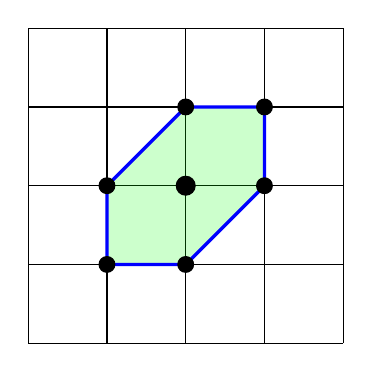
\begin{tikzpicture}
  \draw (0, 0) grid (4, 4);  
\draw [very thick, color=blue, fill=green, fill opacity=0.2]
(1,1) -- (2,1) -- (3,2) -- (3,3) -- (2,3) -- (1,2) -- cycle;
\draw [fill=black]  (1, 1) circle (0.1);
\draw [fill=black]  (2, 1) circle (0.1);
\draw [fill=black]  (3, 2) circle (0.1);
\draw [fill=black]  (3, 3) circle (0.1);s
\draw [fill=black]  (2, 3) circle (0.1);
\draw [fill=black]  (1, 2) circle (0.1);
\draw [fill=black]  (2, 2) circle (0.12);
\end{tikzpicture}
\caption{A hexagon.}
\label{fig:hexagon}
\end{figure}

Consider \cref{fig:hexagon}. It is the $2$-dimensional polytope associated to the del Pezzo surface of degree $6$, whose boundary is exactly the simplicial complex $E_6$. The fan over this polytope correspond to a unimodular regular triangulation of its boundary, and it follows by \cref{eq:unimodular_triangs}, that $\dP6$ degenerates to the Stanley-Reisner ring $\P(E_6 \ast \{pt\})$, where $\{ pt \}$ correspond to the origin. This is an embedded deformation inside $\P^6$.

Now form the join of two copies of $\dP6$, to get a new variety $Y$. By \cref{lemma:join}, this is a $2+2+1=5$-dimensional toric variety with singular locus consisting of two copies of $\dP6$. Since the coordinate ring is just the tensor product of two copies of $S(\dP6)$, it follows that $Y$ degenerates to $\P(E_6 \ast \{pt\} \ast E_6 \ast \{ pt \})=\P(\K \ast \Delta^1)$, whose simplicial complex is the simplicial join of two hexagons. 

Since $\P(\K)$ is a complete intersection inside $\P(\K \ast \Delta^1)$,  it follows that $\P(\K)$ deforms to the intersection of two generic hyperplanes inside $Y$. Denote this deformation by $X_0$. Since $Y$ has singular locus of dimension $2$ and degree $6+6=12$, it follows by Bertini's theorem that $X_0$ has twelve isolated singularities $p_i$.

\begin{lemma}
Let $(U,p_i)$ be the germ of $X_0$ at $p_i$. Then $(U,p_i) \simeq (C(\dP6),0)$.
\end{lemma}
\begin{proof}
Locally, $Y$ looks like $\A^2_{a_1,a_2} \times C(\dP6)_{x_i}$, where the subscripts refer to the coordinates. This is the ideal of $Y$ consists of two sets of equations, each defining a smooth toric variety, and smooth toric varieties are isomorphic to $\A^d$ in affine  charts.

The two hyperplanes $h_1$ and $h_2$ can be written as $\sum_P c_P a^P + \sum c_i x_i$, where $P$ ranges over the hexagon corresponding to $\dP6$. The singularities of $Y$ occur when $x_i=0$ for all $i$, and so locally the singularities of $X_0$ occur when $h_1(a,0,\ldots,0)=h_2(a,0,\ldots,0)=0$. By a change of coordinate, we can assume that the singularity occur when $a_1=a_2=0$ (that is, $c_{(0,0)}=0$). 

Then the leading terms of $h_i$ look like $c_{(1,0)}a_1+c_{(0,1)}a_2+\ldots=0$, for generic $c_P$. This let us eliminate $a_1$ and $a_2$ from the equations, since they .....
\todo{Is this true????}
\end{proof}

\todo{Hva mer å si? Nevne eksistens av krepant resolusjon? (19,19)?}

\section[Smoothings of X0]{Smoothings of $X_0$}

We will exploit the fact that the cone over $\dP6$ have two different smoothings two produce three different smoothings of $X_0$. They all come from writing the equations in different formats.

\subsection{The block matrix construction}

Let $E$ be a 3-dimensional vector space. Let $\{e_1,e_2,e_3\}$ be a basis for $E$. Then we can form the vector space $V= (E \otimes E) \oplus (E \otimes E)$, which has dimension $18$. Let $\P^{17}=\P(V)$.

The elements of $\P^{17}$ can be seen as pairs of $3 \times 3$-matrices, not both zero. Let $M$ be the closure of the set of pairs $(A,B)$ where $\rank A = \rank B = 1$.  

If $\P^{17}$ have coordinates $x_1,\ldots,x_{18}$, let $M_1, M_2$ be the matrices
\[
M_1 = \begin{pmatrix}
x_1 & x_2 & x_3 \\
x_4 & x_5 & x_6 \\
x_7 & x_8 & x_9 
\end{pmatrix}\,
\text{ and }
M_1 = \begin{pmatrix}
x_{10} & x_{11} & x_{12} \\
x_{13} & x_{14} & x_{15} \\
x_{16} & x_{16} & x_{17}
\end{pmatrix}.
\]

Then $M$ is defined by the zeroes of the $2 \times 2$-minors of $M_1$ and $M_2$. Note that $M$ is the projective join of two copies of $\mathbb P^2 \times \mathbb P^2 \hookrightarrow \mathbb P^8$. Since the join of two Fano varieties is Fano, it follows that $M$ is a Fano variety with anticanonical sheaf equal to $\OO_{M}(6)$ \todo{do this!!}.

The variety $M$ is $9$-dimensional: the affine cone over $M$, $C(M)$, is equal to $C(\mathbb P^2 \times \P^2) \times C(\mathbb P^2 \times \P^2)$. This variety has dimension $5+5=10$, hence its projectivization $M$ is $9$-dimensional. 

The singular locus of $M$ consists of the pairs $(0,B)$, and $(A,0)$, where $\rank A= \rank B = 1$, hence $\dim \sing M = 4$. By Bertini's theorem, intersecting $M$ with a codimension $6$ hyperplane gives a smooth variety $X_1$.

Note that by putting $x_1=x_5=x_6$ and $x_{10}=x_{14}=x_{17}$, we get the join of two del Pezzos, so we see that $X_1$ deforms to $X_0$. It follows that $X_1$ is a smooth Calabi-Yau.

A \MM computation give us some information about the geometry of $X_1$.
\begin{proposition}
\label{prop:x1euler} 
$X_1$ has topological Euler characteristic $-72$.
\end{proposition}
\begin{proof}
This is a computation in \MM. Since computing the whole cotangent sheaf of $X_1$ is impossible with current computer technology, we make use of standard exact sequences. Let $\mathscr I$ be the ideal sheaf of $M$ in $\P^{17}$. First off, we have the exact sequence
$$
0 \to \restr{\mathscr I/\mathscr I^2}{X} \to \restr{\Omega_\P^1}{X} \to \restr{\Omega_M^1}{X} \to 0.
$$
The \MM command \texttt{eulers} computes the Euler characteristics of generic linear sections of a sheaf $\mathscr F$. Using this command, we find that $\chi(\restr{\mathscr I/\mathscr I^2}{X})=-180$. Using the exact sequence
$$
0 \to \restr{\Omega_\P^1}{X} \to \OO_X(-1)^{18} \to \OO_X \to 0,
$$
we find that the Euler characteristic of $\restr{\Omega_\P^1}{X}$ is $-216=12\cdot 18$. It follows from the first exact sequence that $\restr{\Omega_M^1}{X}$ has Euler characteristic $-36$.

Since $X$ is a complete intersection, the conormal sequence looks like
$$
0 \to \OO_X(-1)^6 \to \restr{\Omega_M}{X}  \to \Omega_X^1 \to 0.
$$
Hence $\chi(\Omega_X^1) = -36+72 = 36$.

It follows that the topological Euler characteristic is $\chi_X = -2\chi(\Omega_X^1)=-72$.
\end{proof}

\todo{heuristic moduli computation?}

%%%%%%%%%%%%
\subsection{The three-tensor construction}

Now let $F$ be a $2$-dimensional vector space with basis $\{f_1,f_2\}$. Then we can form the vector space $V = ((F \otimes F \otimes F)^{\oplus 2})$. Let $\P^{15}=\P(V)$.

The elements of $\P$ are pairs $(A,B)$ of $2 \times 2 \times 2$-tensors, not both zero. 

Let $N$ be the closure of set of pairs $(A,B)$ where both $A$ and $B$ have tensor rank $1$\footnote{An element of $F^\otimes 3$ have rank $1$ if it is a pure tensor. It has rank $k$ if it can be written as a sum of $k$ pure tensors.}. A pure $2 \times 2 \times 2$-tensor can be visualized as a box in $\Z^3$ of unit volume. Let the variables on $\P^{15}$ be $a_{ijk}$ and $b_{ijk}$ for $i,j,k=0,1$. See the diagram in \vref{fig:222tensor}.

\begin{figure}[t]
\centering
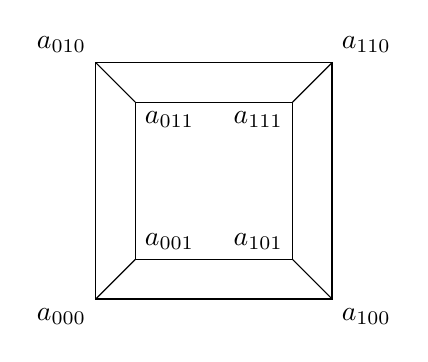
\begin{tikzpicture}
\draw (0,0) -- (3,0) -- (3,3) -- (0,3) -- cycle;
\draw (0.5,0.5) -- (2.5,0.5) -- (2.5,2.5) -- (0.5,2.5) -- cycle;
\draw (0,0) -- (0.5,0.5);
\draw (3,0) -- (2.5,0.5);
\draw (3,3) -- (2.5,2.5);
\draw (0,3) -- (0.5,2.5);
\node[below left] at (0,0) {$a_{000}$};
\node[below right] at (3,0) {$a_{100}$};
\node[above right] at (3,3) {$a_{110}$};
\node[above left] at (0,3) {$a_{010}$};

\node[above right] at (0.5,0.5) {$a_{001}$};
\node[above left] at (2.5,0.5) {$a_{101}$};
\node[below left] at (2.5,2.5) {$a_{111}$};
\node[below right] at (0.5,2.5) {$a_{011}$};
\end{tikzpicture}
\caption{A $2 \times 2 \times 2$-tensor.}
\label{fig:222tensor}
\end{figure}

The equations of the set of rank $1$ tensors are obtained as the ``minors'' along the $6$ sides together with the minors along with the $3$ long diagonals, giving a total of $9$ binomial equations. 

Note that $N$ is the projective join of two copies of $\P^1 \times \P^1 \times \P^1$. As above, it follows that $N$ is a singular Fano variety with anticanonical sheaf equal to $\OO_N(4)$. 

The singular locus of $N$ consists of the pairs $(A,0)$ and $(0,B)$ where both $A,B$ have rank $1$. Hence the singular locus is of dimension $3$.

Intersecting $N$ with a codimension $4$-hyperplane gives a smooth variety $X_2$. It is Calabi-Yau and has topological Euler characteristic $-48$.

\begin{proposition}
The topological Euler characteristic of $X_2$ is $-48$.
\end{proposition}
\begin{proof}
The proof is identical to the proof of \cref{prop:x1euler}.
\end{proof}

\subsection{The mixed smoothing}

In the above cases, we formed the join of equal varieties. In tha above notation, let $V=(E \otimes E) \oplus (F \otimes F \otimes F)$. Then let $\P^{16}=\P(V)$.

Now let $W$ be the set of ``mixed'' rank $1$ tensors. In a way similar to above, we find that $W$ is a singular Fano toric variety of dimension $8$. The singular locus is of dimension $4$, so a $5$-fold complete intersection is again a smooth Calabi-Yau variety $X_3$.

\begin{proposition}
The Euler characteristic of $X_3$ is $-60$.
\end{proposition}
\begin{proof}
The proof is identical to the proofs above.
\end{proof}


%%%%%%%%%%%%%%%
\section{Invariant \CY's}

By choosing non-generic hyperplanes in the construction of $X_1$ and $X_2$, there will be natural group actions on them.

Denote by $D_6$ the dihedral group of order $12$, the symmetries of a hexagon. It is generated by a rotation $\rho$ of order $6$, together with a reflection $\sigma$, subject to $\sigma \rho \sigma = \rho^{-1}$. There is an isomorphism $D_6 \simeq S_3 \times \Z_2$ given by the inclusion $S_3 = \langle \rho^2, \sigma \rangle \hookrightarrow D_6$. 


\begin{lemma}
There are $D_6$-actions on both $M$ and $N$.
\end{lemma}
\begin{proof}
Recall that $M$ is the join of two copies of $\P^2 \times \P^2$ embedded in $\P^8$. We can think of $M$ as the rank $1+1$ block matrices in $\P(E \otimes E \oplus E \otimes E)$, where $E$ is a $3$-dimensional vector space. Choosing a basis $\{e_1,e_2,e_3\}$ for $E$, we have a natural $S_3$ action on $E$ given by $e_i \mapsto e_{\sigma(i)}$. This action extends to $E \otimes E$. 

Switching the direct summands of ${\left(E \otimes E\right)}^{\oplus 2}$, gives us a $\Z_2$-action. In total we now have a $S_3 \times \Z_2$-action, which by the above remark is a $D_6$-action. Note that since the action was defined on $E$, rank is preserved, so that we indeed have an action on $M$.

Similarly, $N$ is the rank $1+1$ tensors in ${\left(E \otimes E \otimes E \right)}^{\oplus 2}$, where now $E$ is a $2$-dimensional vector space. 
\end{proof}

\todo{Torus actions}

By choosing invariant hyperplanes, the group actions on the ambient spaces descend to the \CY's. We first consider the case when the ambient space was the join of two copies of $\P^2 \times \P^2$, which was denoted by $M$ above.

Denote a unit matrix in the first factor of $(E \otimes E) \oplus (E \otimes E)$ by $e_{ij}^0$, and denote a unit matrix in the second factor by $e_{ij}^1$, where $0,1$ are taken modulo $2$. 

In this case, one such invariant hyperplane is given by the span of
$$
f_{ij}^\alpha = e_{ij}^\alpha + t e_{-i-j,-i-j}^{\alpha+1} \in E\otimes E \oplus E \otimes E,
$$
where $i \neq j \in \Z_3$ and $\alpha \in \Z_2$. Denote the intersection between $M$ and $H$ by $X_{H_t}$. Then the following is true:

\begin{proposition}
Both the finite group $D_6$ and the group $\Z_3$ act on $X_{H_t}$. The symmetric variety $X_{H_t}$ have $24$ isolated singularities for $t \neq 0,1$, and they come in two orbits under the $D_6$-action.

For $t=1$, it has $36$ isolated singularities.
\todo{Check \emph{which} singularities these are, also: fix points}
\end{proposition}

There is also a torus action on $E$, defined by $e_i \mapsto \omega^i e_i$, where $\omega$ is a third root of unity. This a $\Z/3$-action, which extends to an action on $ E\otimes E \oplus E \otimes E$. Let $H=\Z/3$. Then note that $X_{H_t}$ is $\Z/3$-invariant as well. 

\todo{identify $H$-invariant singularities + fix points}




\section{Euler characteristic heuristics}

\begin{enumerate}
	\item By a naive count, things make sense
\end{enumerate}

